\documentclass[a4paper,12pt]{article}
\usepackage[utf8]{inputenc}
\usepackage[brazil]{babel}
\usepackage[parfill]{parskip} % Activate to begin paragraphs with an empty line rather than an indent

\usepackage{graphicx} % support the \includegraphics command and options
\usepackage{url} % support the url references

\usepackage{fancyvrb} % better looking verbatim

\usepackage{float}

%font
\usepackage{times}
% \usepackage{mathptmx}
\usepackage[T1]{fontenc}

% to adjust figures numbering
% \usepackage{amsmath}
% \numberwithin{figure}{section}

% %figura
% \begin{figure}[h]
% \centering
% \includegraphics[width=\linewidth]{imgs/.png}
% \label{fig:}
% \caption{}
% \end{figure}


\author{Alberto Vital Santos de Sousa}

\begin{document}
%================CAPA===================
\pagenumbering{gobble} % turn off page numbering
\begin{center}
\begin{figure}[h]
\centering

\includegraphics[width=3cm]{imgs/ufpe.png}

\includegraphics[width=4cm]{imgs/cin.png}
\end{figure}
%{\Large
Universidade Federal de Pernambuco\\
Centro de Informática\\
Curso de Bacharelado em Engenharia da Computação
%}
\\[3cm]
\textbf{\huge
AndroidDriller:\\[3mm]
Uma ferramenta de mineração de repositórios Android\\
}
\vfill
\begin{flushleft}
Aluno: Alberto Vital Santos de Sousa\\
Orientador: Leopoldo Motta Teixeira\\[5mm]
\end{flushleft}
Recife, junho de 2018
\end{center}

%================ContraCapa===================
\newpage
\begin{center}
Universidade Federal de Pernambuco\\
Centro de Informática\\
Curso de Bacharelado em Engenharia da Computação
%}
\\[3cm]
\textbf{\huge
AndroidDriller:\\[3mm]
Uma ferramenta de mineração de repositórios Android\\
}
\vfill

\begin{flushleft}
{\small
Monografia apresentada ao Centro de Informática (CIn)\\
da Universidade Federal de Pernambuco (UFPE), como requisito\\
parcial para conclusão do Curso de Engenharia da Computação,\\
orientada pelo professor Leopoldo Motta Teixeira.
}
\end{flushleft}
Recife, junho de 2018
\end{center}


%================AGRADECIMENTOS===================
\newpage
\section*{Agradecimentos}

%São muitos nomes para que eu me lembre de todos os que merecem aqui, mas gostaria de agradecer àqueles que de alguma forma contribuíram não só para este trabalho como também para a minha formação como pessoa. Em especial posso citar meus pais Antonio Vital Alves de Sousa e Maria Auxiliadora Santos Vital Alves de Sousa, que sempre me apoiaram e me incentivaram nas minhas decisões e a sempre seguir com meus estudos. Também agradeço ao meu orientador Leopoldo Motta Teixeira, pelos ensinamentos que me proporcionou durante este período. De uma maneira geral agradeço também a todos os meus colegas de graduação e do laboratório Oki Brasil, que estiveram ao meu lado durante os momentos difíceis da graduação e também nos de  descontração do dia a dia.

%================RESUMO===================
\newpage
\pagenumbering{arabic} % turn page numbering back on
\section*{Resumo}
Utilizando ferramentas capazes de minerar dados sobre repositórios, pesquisadores de engenharia de software têm obtido um melhor conhecimento sobre o processo de desenvolvimento de software, em geral. Este trabalho propõe uma ferramenta capaz de minerar repositórios fazendo uso das características comuns de projetos Android para que se possa realizar uma investigação preliminar de como as mudanças acontecem no desenvolvimento de aplicações para a plataforma.

\textbf{Palavras-chave}: Android, Mineração de Repositórios, Sistema de Controle de Versão, Git

%================ABSTRACT===================
\newpage
\section*{Abstract}

Software Engineering researchers have been using tools capable of mining data from repositories to get a better understanding about the software development process. This work proposes a tool for mining repositories that uses the common characteristics of Android Projects so we can perform a preliminary investigation about how changes occur in the platform apps development.

\textbf{Keywords}: Android, Repository Mining, Version Control System, Git

%================Sumario===================
\newpage

\tableofcontents

%================INTRODUÇÃO===================
\newpage
\section{Introdução}

Em engenharia de software, a análise de repositórios tem ajudado pesquisadores a
obter um melhor conhecimento sobre o processo de desenvolvimento de um
software \cite{miningGit}. Com isso, é possível predizer bugs e também analisar o padrão de
desenvolvimento utilizado pelos colaboradores do projeto. Para tal fim, existem
ferramentas capazes de minerar dados sobre repositórios, como por exemplo, o
RepoDriller \cite{repodriller}.\\
\\
Ferramentas mais gerais, como o próprio RepoDriller, servem para analisar
software em vários domínios. No desenvolvimento de aplicações Android, há
diversas particularidades envolvidas. Por exemplo, o arquivo de manifesto contém
informações sobre os vários componentes do projeto. Assim, as principais
alterações feitas no repositório são refletidas em modificações desse arquivo.\\
\\
No estudo de repositórios Android, pesquisadores têm usado ferramentas capazes
de extrair dados dos arquivos do tipo apk \cite{Calciati}, \cite{WhoAdded} e \cite{YLyu}. Para realizar estudos
semelhantes, uma outra abordagem seria utilizar uma ferramenta capaz de
minerar os repositórios das aplicações e extrair dados específicos levando em
consideração não só o arquivo apk mas também as modificações dos arquivos de
manifesto, por exemplo.\\


%================OBJETIVOS===================

\subsection{Objetivos}

Este trabalho tem por objetivo realizar uma investigação preliminar de como as
mudanças acontecem no desenvolvimento de aplicações Android para criar
ferramentas de suporte à evolução de aplicativos, e assim, implementar uma
ferramenta capaz de minerar estes repositórios, aproveitando-se das
características particulares de projetos Android.\\


%=============================
%=      Desenvolvimento      =
%=============================

%================CONCEITOSBASICOS===================
\newpage

\section{Conceitos Básicos}

Neste capítulo apresentamos conceitos essenciais para a compreensão do trabalho. Na seção \ref{sec:android} apresentamos a plataforma Android e seus componentes. Na seção \ref{sec:scv} explicamos o que são sistemas de controle de versão, destacando o Git.  Na seção seguinte comentamos sobre mineração de repositórios, e por fim, ainda na seção \ref{sec:mining}, apresentamos o framework utilizado para desenvolver a ferramenta proposta.

\subsection{Android}%10
%o que é android
\label{sec:android}
O sistema operacional Android pode ser definido como uma pilha de software de código aberto desenvolvida para sistemas móveis \cite{androidSource}. A partir desta pilha, programadores são capazes de desenvolver aplicações para dispositivos móveis sem se preocupar com detalhes específicos de hardware, pois a própria plataforma trata essas diferenças em sua API. O fato de Android ter seu código aberto, também permite ao desenvolvedor implementar sua própria versão dos módulos da plataforma caso deseje.

A pilha de software citada acima pode ser dividida em camadas, conforme a figura \ref{fig:androidStack}

%figura dos modulos
\begin{figure}[h]
\centering
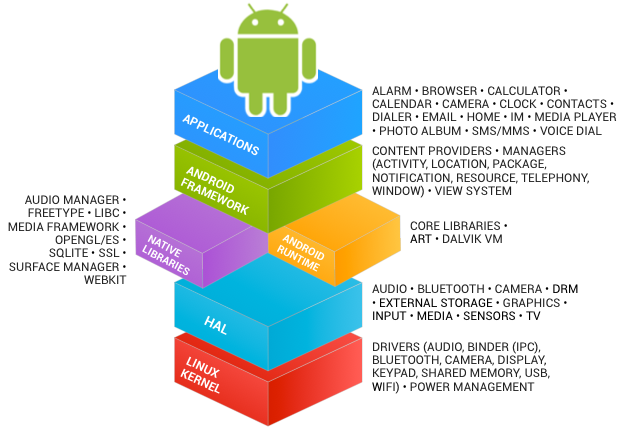
\includegraphics[width=0.8\linewidth]{imgs/android_framework_details.png}
\caption{Pilha de software dividida em camadas \cite{androidSource}}
\label{fig:androidStack}
\end{figure}

Este trabalho propõe uma ferramenta para extrair dados relativos à camada \textit{Applications}, onde estão as aplicações e as principais classes utilizadas pelos desenvolvedores para produzi-las. Mais abaixo trataremos alguns dos principais elementos da plataforma e que são abordados pela ferramenta proposta.

%detalhamento dos componentes
%olhar pagina do android developer
\subsubsection{AndroidManifest}
%O core da ferramenta
É um arquivo XML obrigatório que contém informações sobre os componentes da aplicação. Precisa ser criado com o nome \textit{AndroidManifest.xml}, dessa forma a plataforma é capaz de identificar, dentre outras coisas, qual parte do código implementa a cada uma das entidades que compõem a aplicação. Um exemplo desse arquivo pode ser visto na figura \ref{fig:manifest}.

 %figura de manifesto
 \begin{figure}[h]
 \centering
 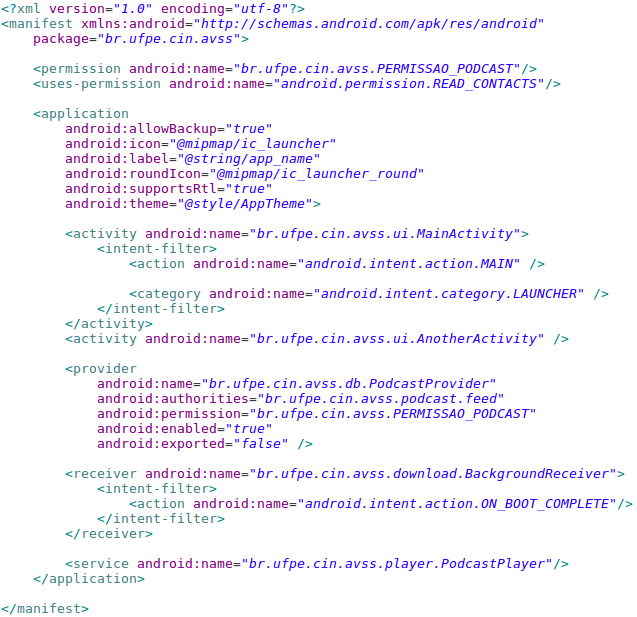
\includegraphics[width=\linewidth]{imgs/manifest.png}
 \caption{Exemplo de arquivo AndroidManifest.xml}
 \label{fig:manifest}
 \end{figure}



\subsubsection{Activity}
Representa a interface visual de interação com o usuário. No arquivo de manifesto é representada pela tag \textit{activity} e precisa definir o atributo \textit{name}, que é utilizado para identificar a classe que a implementa.\\

Na figura \ref{fig:manifest} podemos ver duas activities sendo declaradas, uma delas possui o atributo \textit{name} definido como \textit{br.ufpe.cin.avss.ui.AnotherActivity}.
{\fontsize{9pt}{12pt}
\begin{Verbatim}
<activity android:name="br.ufpe.cin.avss.ui.AnotherActivity" />
\end{Verbatim}
}

Dessa forma, a plataforma espera encontrar no pacote \textit{br.ufpe.cin.avss.ui} a implementação da classe AnotherActivity que representará uma das telas da aplicação.

\subsubsection{Broadcast Receiver}

A plataforma Android utiliza um sistema de eventos similar ao padrão \textit{publish-subscribe}, onde a plataforma (ou outra aplicação) dispara um evento (\textit{broadcast}) e as aplicações registradas para o evento recebem a mensagem correspondente. O componente que recebe estes eventos é conhecido como \textit{broadcast receiver}.\\
Ao iniciar o dispositivo, o sistema android dispara um evento de \textit{broadcast} chamado de ON\_BOOT\_COMPLETE. Para que a aplicação receba esse e outros eventos semelhantes é necessário implementar uma classe do tipo \textit{Broadcast Receiver} e registrá-la no evento desejado. Para isso, declara-se no manifesto a tag \textit{receiver}, conforme o trecho abaixo, que também pode ser visto na figura \ref{fig:manifest} onde foi declarado um componente receiver que espera eventos do tipo citado anteriormente.
{\fontsize{9pt}{12pt}
\begin{verbatim}
<receiver android:name="br.ufpe.cin.avss.download.BackgroundReceiver">
  <intent-filter>
    <action android:name="android.intent.action.ON_BOOT_COMPLETE"/>
  </intent-filter>
</receiver>
\end{verbatim}
}

\subsubsection{Content Provider}
\label{sec:provider}
Componente responsável por prover uma interface de acesso para outras aplicações aos dados utilizados. Dessa forma, cria-se uma abstração da camada de dados que pode ser utilizada não só por outras aplicações como também pela própria aplicação, conectando os dados em um processo com o código em execução em outro.\\

No manifesto é representada pela tag \textit{provider}. Na figura \ref{fig:manifest} temos um exemplo que foi replicado no trecho abaixo, onde a exemplo da tag activity, o atributo name define a classe com a implementação correspondente.
{\fontsize{9pt}{12pt}
\begin{verbatim}
<provider
    android:name="br.ufpe.cin.avss.db.PodcastProvider"
    android:authorities="br.ufpe.cin.avss.podcast.feed"
    android:permission="br.ufpe.cin.avss.PERMISSAO_PODCAST"
    android:enabled="true"
    android:exported="true" />
\end{verbatim}
}

Ao declarar este elemento é necessário definir o atributo \textit{authorities}, que seguindo a convenção de nomes em Java, identifica o provider declarado.\\

O atributo \textit{permission} define que para acessar os dados deste receiver, é necessário possuir a permissão \textit{br.ufpe.cin.avss.PERMISSAO\_PODCAST}, um elemento que será discutido mais à frente.




\subsubsection{Service}



Este componente não provê uma interface visual e roda em background. Dessa forma, é utilizado para implementar procedimentos  que não necessitam que a aplicação esteja ativa no momento. Em geral, operações mais pesadas como downloads de arquivos e reprodução de áudio são realizadas por estes componentes, uma vez que sua execução não é finalizada mesmo quando o usuário sai da aplicação. No manifesto é declarado com a tag \textit{service}, como pode ser visto no trecho abaixo retirado da figura \ref{fig:manifest}.
{\fontsize{9pt}{12pt}
\begin{verbatim}
<service android:name="br.ufpe.cin.avss.player.PodcastPlayer"/>
\end{verbatim}
}

\subsubsection{Permission}
%tratar uses-permission aqui
O sistema de permissões da plataforma Android garante que certas ações só sejam executadas caso o usuário da aplicação conceda o privilégio necessário. Dessa forma, caso uma aplicação deseje ler os contatos do usuário, por exemplo, é necessário declarar a tag \textit{uses-permission} no manifesto com o atributo \textit{name} de valor igual a "android.permission.READ\_CONTACTS", conforme pode ser visto na figura \ref{fig:manifest}.

{\fontsize{9pt}{12pt}
\begin{verbatim}
<uses-permission android:name="android.permission.READ_CONTACTS"/>
\end{verbatim}
}

%tratar das dangerous
As permissões podem ser classificadas em:
\begin{itemize}
    \item {Dangerous}
    \item {Normal}
    \item {Signature}
    \item {Signature or System}
\end{itemize}

As permissões consideradas \textit{dangerous} podem causar algum risco à privacidade do usuário ou ao funcionamento normal do dispositivo, por isso necessitam da validação do usuário. As \textit{normal}, por não trazerem esses riscos, são concedidas automaticamente pelo sistema ao serem declaradas no manifesto.\\

Desde a versão 6.0 da plataforma android, a forma como as permissões são solicitadas foi alterada. Nas versões anteriores, qualquer permissão \textit{dangerous} é solicitada antes da instalação, e caso a aplicação precise ser atualizada, as permissões são solicitadas novamente. Caso o usuário não conceda alguma permissão, a aplicação não é instalada nem atualizada. A partir da versão 6.0, as permissões \textit{dangerous} são solicitadas em tempo de execução. Dessa forma, a aplicação pode ser instalada sem que o usuário tenha que conceder todos os privilégios solicitados. Assim,  a permissão associada com a funcionalidade ativada é solicitada sempre que o usuário desejar utilizar a funcionalidade.\\

%tratar das permissoes criadas pela aplicação
Existe também a possibilidade da própria aplicação definir permissões de acesso ao seus conteúdos. Para isso, utiliza-se a tag \textit{permission}. Conforme foi visto na seção \ref{sec:provider}, o atributo \textit{permission} pode ser utilizado para definir uma permissão de acesso ao conteúdo provido pelo componente. Dessa forma, pode-se notar que a aplicação definida no arquivo da figura \ref{fig:manifest} não só define uma permissão própria, como também protege seu content provider com essa mesma permissão, de acordo com as tags do trecho abaixo.

{\fontsize{9pt}{12pt}
\begin{verbatim}
<permission android:name="br.ufpe.cin.avss.PERMISSAO_PODCAST"/>
...
<provider
    android:name="br.ufpe.cin.avss.db.PodcastProvider"
    android:authorities="br.ufpe.cin.avss.podcast.feed"
    android:permission="br.ufpe.cin.avss.PERMISSAO_PODCAST"
    android:enabled="true"
    android:exported="false" />
\end{verbatim}
}



%\newpage
\subsection{Sistemas de controle de versão}%11-15
\label{sec:scv}
São sistemas que controlam o versionamento de um software durante o estágio de desenvolvimento. Com estes sistemas é possível saber qual o estado exato do código fonte em um determinado período do processo de produção, pois a cada alteração realizada o SCV armazena quais arquivos e quais linhas foram modificadas naquele momento, além de também informar quem realizou as alterações.

\subsubsection{Git}%11-17
%\newpage
É um sistema de controle de versão descentralizado livre e de código aberto \cite{git}, onde cada desenvolvedor tem uma cópia completa do histórico do repositório. A cada conjunto de  alterações registrada  um \textit{snapshot} do projeto denominado \textit{commit} é armazenado. O git utiliza uma estrutura de grafos para organizar os commits em diversas linhas de desenvolvimento, cada uma sendo denominada \textit{branch} \cite{gitHandbook}.

Abaixo estão listados alguns dos principais comandos git, juntamente com uma breve explicação de seu funcionamento.

\begin{itemize}
\item{\textit{git init} } Inicializa um repositório a partir de um diretório local.
\item{\textit{git clone} } Copia um repositório remoto em um diretório local.
\item{\textit{git pull} } Recupera as mudanças remotas para o repositório local.
\item{\textit{git add} } Adiciona as mudanças locais num conjunto para que possam ser incluídas no próximo commit.
\item{\textit{git commit} } Cria um commit com as mudanças selecionadas pelo comando git add.
\item{\textit{git push} } Atualiza o repositório remoto remoto com as mudanças locais.
\item{\textit{git branch} } Cria uma nova linha de desenvolvimento
\item{\textit{git merge} } Unifica duas linhas de desenvolvimento em um novo commit que é denominado \textit{merge commit}
\end{itemize}

Para exemplificar o funcionamento de um merge commit, suponha o seguinte grafo de commits de um repositório representado pela figura \ref{fig:graphBefore}.

 %figura
 \begin{figure}[h]
 \centering
 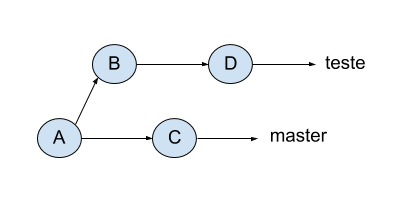
\includegraphics[width=0.65\linewidth]{imgs/graph_before.png}
 \caption{Grafo de commits com duas branches}
 \label{fig:graphBefore}
 \end{figure}



Estando na branch master e executando o comando \textit{git merge teste} cria-se o commit \textit{E} na branch master e que unifica as modificações realizadas nas duas branches, resultando no grafo da figura \ref{fig:graphAfter}.

 %figura
 \begin{figure}[H]
 \centering
 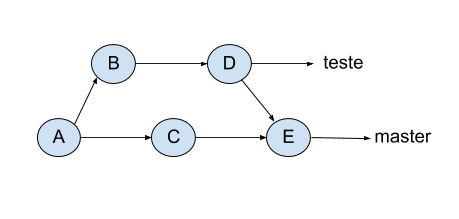
\includegraphics[width=0.65\linewidth]{imgs/graph_after.png}
 \caption{Grafo de commits após o merge commit 'E'.}
 \label{fig:graphAfter}
 \end{figure}


\subsection{Mineração de repositórios}%11-15
\label{sec:mining}



A análise de software consiste em extrair dados para que gerentes e engenheiros de software possam melhorar o processo de desenvolvimento de software através do ganho e compartilhamento de ideias provenientes desses dados para uma melhor tomada de decisão \cite{soWhat}. Dessa forma, podemos definir como mineração de repositórios o processo de  extração desses dados. Devido ao tamanho e a quantidade de repositórios utilizados durante seus estudos, pesquisadores têm utilizado ferramentas de mineração para automatizar esse processo. %\cite{something I don't know yet}.
\\
\\
Na próxima seção apresentamos uma ferramenta utilizada para minerar repositórios, e que foi utilizada como base para a ferramenta desenvolvida neste trabalho.

%%%%%%%%%
%citar crescente dos dados -> uso de ferramentas de mineração.

%\newpage
\subsubsection{RepoDriller}%14-16
\label{sec:repodriller}
Repodriller é um framework de mineração de repositórios feito em Java  \cite{repodriller}. Com esta ferramenta é possível extrair dados não só dos commits realizados (como por exemplo autor e mensagem) mas também dos arquivos contidos no repositório.

Para escrever um programa que minere um dado repositório, é preciso implementar a interface \textit{Study} e no método \textit{execute} criar um objeto de estudo (uma instância da classe \textit{RepositoryMining}) utilizando o padrão builder e informando além do repositório a ser minerado, as implementações da interface \textit{CommitVisitor}.  Para informar o repositório, utilizamos o método \textit{in} que recebe uma implementação de  \textit{SCMRepository}, podendo ser tanto Git quanto SVN. Neste trabalho foi utilizado a implementação \textit{GitRemoteRepository} que recebe uma URL referenciando o repositório remoto, ver figura \ref{fig:repostudy}.

A interface \textit{CommitVisitor} define o método \textit{process} que é chamado pela API interna do RepoDriller a cada commit visitado. O método \textit{process} recebe como parâmetros \textit{SCMRepository}, \textit{Commit} e \textit{PersistenceMechanism}. O primeiro é um objeto representando o repositório estudado, podendo ser Git ou SVN. O segundo é uma representação do commit sendo visitado. E o terceiro é um objeto para tratar a persistência dos dados minerados ao longo dos vários commits visitados.

Ainda no objeto \textit{RepositoryMining}, definimos o mecanismo de persistência a ser passado para cada visitor. Em geral, escolhe-se um arquivo CSV. A partir da versão 1.4 do RepoDriller, pode-se definir uma configuração de coleta, para evitar que dados desnecessários sejam carregados a cada commit. Para o nosso caso em que vamos focar em informações básicas do commit e nas modificações do arquivo de manifesto, foi acrescentada a linha \textit{.collect(new CollectConfiguration().basicOnly().sourceCode().diffs())} como pode ser visto na figura \ref{fig:repostudy}.


%figura do objeto RepositoryMining.
\begin{figure}[h]
\centering
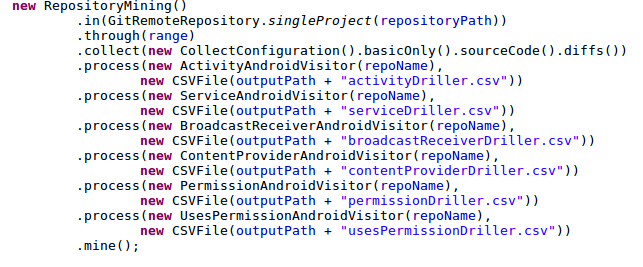
\includegraphics[width=\linewidth]{imgs/repostudy.png}
\caption{Objeto RepositoryMining definido no método \textit{execute} da classe RepoStudy.}
\label{fig:repostudy}
\end{figure}



%================FERRAMENTA===================
\newpage
\section{AndroidDriller}%18-24
%Detalhamento geral da ferramenta

Neste capítulo apresentamos a ferramenta desenvolvida ao longo deste trabalho. Na seção \ref{sec:metodologia} descrevemos o processo geral do que foi desenvolvido. Na seção \ref{sec:implementacao} detalhamos cada classe implementada. Em seguida, na seção \ref{sec:repoteste} comentamos sobre os repositórios escolhidos para validar e testar a implementação. Por fim, nas seções \ref{sec:experimentos} e \ref{sec:resultados} explicamos um experimento onde foram extraídos dados de repositórios Android com o AndroidDriller  e os resultados obtidos, respectivamente.

\subsection{Metodologia}
\label{sec:metodologia}
Foi criada uma ferramenta Java que faz uso da API provida pelo RepoDriller para
percorrer os commits do repositório. Neste projeto foram implementadas as
classes capazes de colher dados sobre os componentes específicos de Android e
geração de relatórios em arquivos CSV. Para visualização dos dados, foi
implementado um programa na linguagem Python capaz de produzir gráficos a
partir dos arquivos CSV gerados pela ferramenta. Este fluxo pode ser descrito pela figura \ref{fig:workflow}.

 %figura
 \begin{figure}[h]
 \centering
 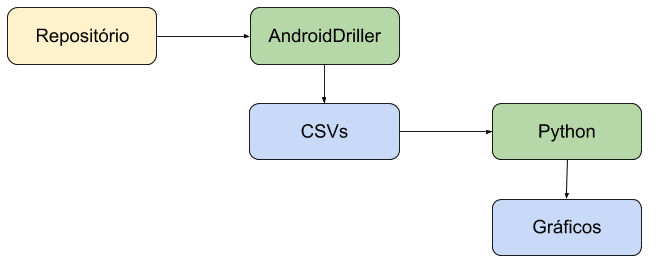
\includegraphics[width=0.65\linewidth]{imgs/workflow.png}
 \caption{Fluxo dos dados de um repositório até os gráficos gerados.}
 \label{fig:workflow}
 \end{figure}



\subsection{Implementação}%18-24
\label{sec:implementacao}


Primeiramente, vamos apresentar o modelo utilizado para representar as entidades da plataforma Android. Como pode ser visto na figura \ref{fig:model}, temos uma classe que representa o arquivo de manifesto e cada elemento do XML foi mapeado em uma classe Java. Para representar os componentes foi utilizado o padrão de herança entre classes. Dessa forma, a classe \textit{Component} contém os atributos comuns aos componentes Android, que foram representados cada um com uma classe filha de Component.\\

%figura do diagrama do modelo
\begin{figure}[H]
\centering
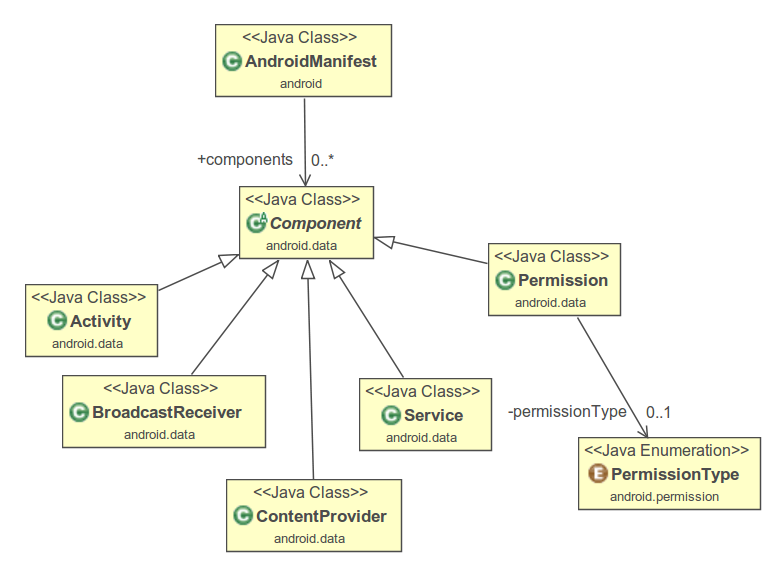
\includegraphics[width=0.8\linewidth]{imgs/model.png}
\caption{Diagrama das classes de modelo da plataforma Android.}
\label{fig:model}
\end{figure}


A classe Component também define o método \textit{isModificationOf} que recebe outro componente e verifica se um é apenas uma modificação do outro ou se são componentes totalmente distintos. Para fazer essa verificação foi utilizado o atributo name como identificador do componente, ou seja, se dois componentes têm o mesmo valor de name mas valores diferentes para outros atributos, eles representam o mesmo componente apenas modificado, mas se dois componentes têm os mesmos valores de todos os atributos e diferem apenas no valor do name, eles representam componentes distintos. Dessa forma, cada uma das subclasses de Component podem sobrescrever este método e acrescentar seus atributos específicos. Este método será útil mais à frente quando comentarmos sobre a classe \textit{ComponentDiff}.

Por conveniência, os atributos e métodos foram omitidos dos diagramas aqui apresentados. %No apêndice encontram-se mais detalhes da estruturas das classes.


Seguindo uma arquitetura semelhante à das classes de modelo, foram implementadas classes de diff, conforme a figura \ref{fig:diff}. Essas classes tratam o diff específico de cada componente. \\


%figura do diagrama dos diffs
\begin{figure}[h]
\centering
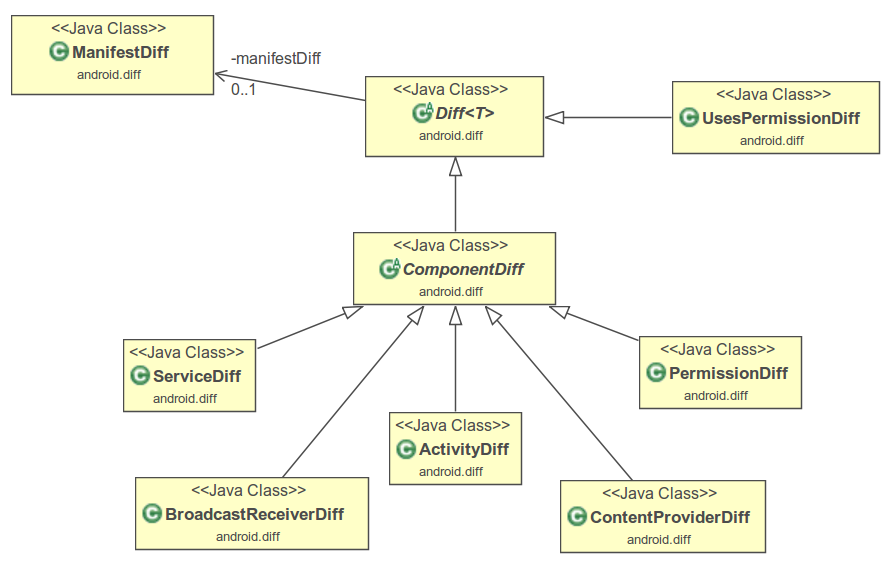
\includegraphics[width=0.8\linewidth]{imgs/diff.png}
\caption{Diagrama das classes que tratam as alterações de cada commit.}
\label{fig:diff}
\end{figure}


A classe ManifestDiff recebe uma lista de modificações registradas em cada commit, dessa lista, são filtradas as que se referem a qualquer arquivo com a denominação AndroidManifest.xml. A partir das alterações  nos manifestos, são criadas duas listas de versões dos arquivos, uma lista de arquivos anteriores e outra posteriores ao commit. De posse dessas versões utilizamos a classe AndroidManifestParser para criar duas listas de instâncias da classe AndroidManifest definida pelo modelo. As instâncias de AndroidManifest são então passadas para a classe parametrizada abstrata Diff<T> . \\

De uma forma geral, em Diff são criadas duas listas de componentes, uma representando os componentes anteriores ao commits e outra os posteriores. A partir disso, mais três listas são criadas, uma com as adições, outra com as remoções e a terceira com os componentes modificados. Para reusar o código definido nesta classe, o parâmetro T define qual componente será analisado pela subclasse de Diff, pois esta define o método abstrato \textit{getElementsList} que recebe uma instância do  retorna uma lista de objetos do tipo T. A classe também define outro método abstrato, \textit{isModification}, que recebe um elemento T e verifica se ele foi modificado. Dessa forma, as subclasses só precisam implementar estes dois métodos para que se possa obter informações específicas de cada componentes desejado. \\

Note que na figura \ref{fig:diff} a classe UsesPermissionDiff herda diretamente da classe Diff, enquanto que os outros componentes herdam da classe ComponentDiff. Isto ocorre porque o elemento uses-permission só define um atributo do tipo String, por isso, ele é representado apenas como uma String com o valor desse atributo. Por esta mesma razão este componente não está representado no diagrama de modelo da figura \ref{fig:model}. Enquanto isso, a classe abstrata ComponentDiff define o parâmetro T para ser o tipo Component, implementando o método getElementsList para retornar uma lista de Component que é recuperada pelo método abstrato \textit{getComponents}, e também implementa o método isModification para retornar o isModificationOf  definido pela instância de Component, conforme vimos anteriormente. Assim as subclasses podem implementar apenas o método getComponents de forma mais específica.

%diagrama de classes
Como visto anteriormente, para percorrer os commits de um dado repositório, é preciso implementar uma interface provida pelo RepoDriller. Para que se pudesse utilizar a mesma implementação para os vários repositórios a serem minerados, foi criada a classe \textit{RepoStudy}, que implementa a interface \textit{Study}, conforme figura \ref{fig:study}.

%diagrama do objeto repostudy.
\begin{figure}[h]
\centering
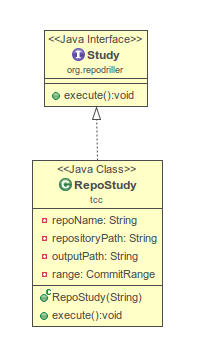
\includegraphics[width=0.3\linewidth, height=0.45\linewidth]{imgs/study.png}
\caption{Diagrama de classe do objeto RepoStudy.}
\label{fig:study}
\end{figure}

Essa classe recebe a url do repositório a ser estudado e a partir disso inicializa o objeto \textit{RepositoryMining} com o repositório a ser minerado e registra os visitors específicos de repositórios android que serão mais detalhados à frente.


A exemplo do que foi visto na seção \ref{sec:repodriller}, para que possamos analisar cada commit, foram implementados visitors que extraem dados a respeito de cada componente separadamente. Esses visitors seguem a estrutura definida na figura \ref{fig:visitors}, onde um visitor abstrato implementa a interface CommitVisitor definida pelo RepoDriller, repassando a chamada do método process (que recebe um Commit) da interface para o método abstrato androidProcess (que recebe um AndroidCommit) conforme figura \ref{fig:diagram}. Dessa forma, o Commit provido pelo framework é convertido em uma instância de \textit{AndroidCommit}. Assim, a classe DiffAndroidVisitor implementa o método androidProcess e define o método abstrato \textit{getDiff}, repassando o AndroidCommit para as subclasses retornarem cada uma a instância da classe de diff do componente correspondente. Ainda no método androidProcess, são registrados os dados recuperados pela subclasse de Diff, retornada pelo método getDiff, no arquivo CSV definido pelo visitor utilizando a instância de PersistenceMechanism passada.

A classe AndroidCommit estende a classe Commit do RepoDriller, adicionando informações específicas Android. No seu construtor, esta classe recebe o commit a ser estendido e o repositório a qual ele pertence, parâmetros que são utilizados para recuperar os manifestos do commit e a lista de modificações. A partir disso, é possível criar uma instância de ManifestDiff, que é utilizada como base para criação das instâncias das subclasses de Diff que serão recuperadas pelos visitors específicos, como visto anteriormente.


%figura dos visitors
\begin{figure}[h]
\centering
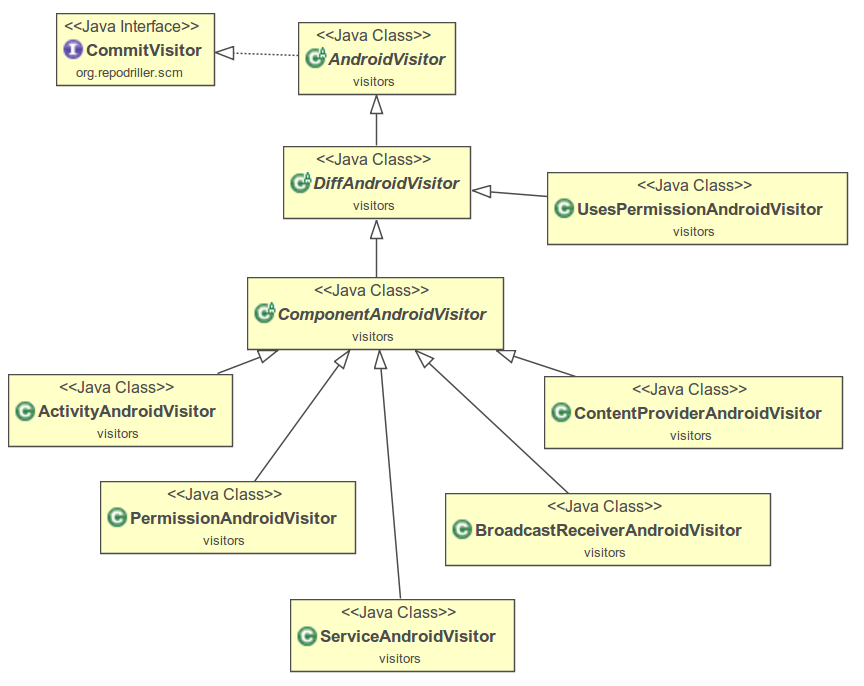
\includegraphics[width=0.8\linewidth]{imgs/visitors.png}
\caption{Diagrama das classes que implementam os visitors de cada componente.}
\label{fig:visitors}
\end{figure}


%figura do diagrama .
\begin{figure}[h]
\centering
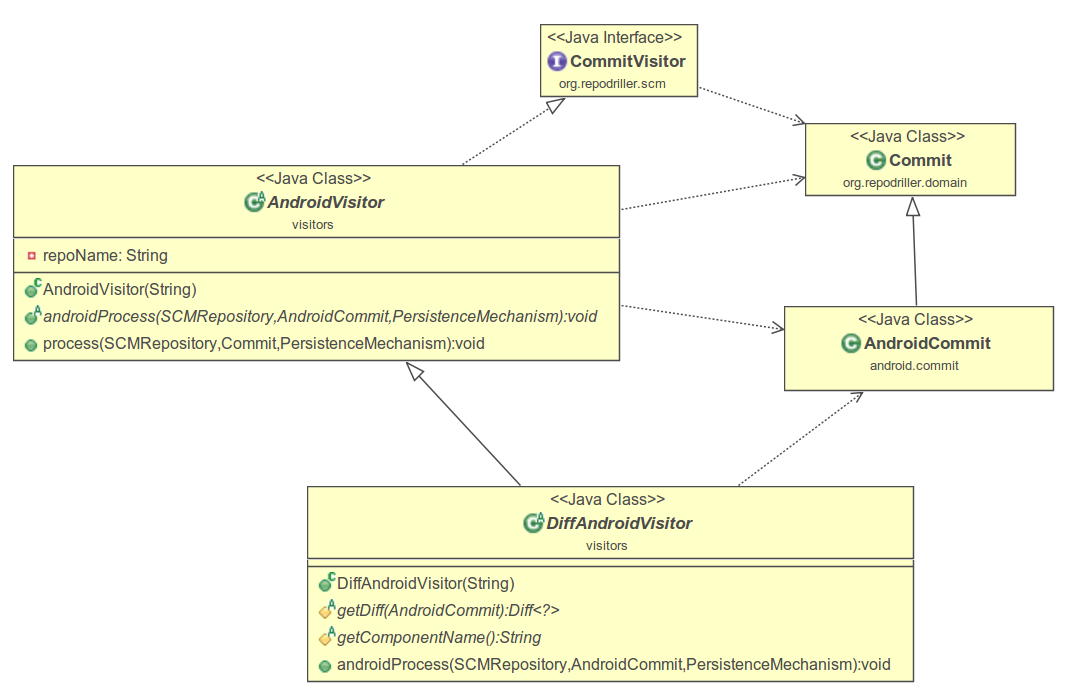
\includegraphics[width=\linewidth]{imgs/diagram.png}
\caption{Diagrama do encapsulamento do método process e da classe Commit.}
\label{fig:diagram}
\end{figure}


Para que tudo isto funcione, foi implementada a classe MyStudy, que no seu método main,  lê o arquivo de entrada encontrado na pasta androidDriller/input com o nome repoURLs.in. Este arquivo deve conter uma lista de URLs de repositórios Android remotos do github. Para cada repositório, a classe MyStudy cria uma instância de RepoStudy passando a URL do repositório como parâmetro. Na classe RepoStudy, é criado o diretório de saída, androidDriller/output, no qual são criadas uma pasta para cada repositório minerado,  onde se encontrarão os arquivos CSV gerados. 


%================repositórios de teste===================
\subsection{Repositórios de Teste}%18-22
\label{sec:repoteste}

No intuito de gerar um cenário pequeno, com poucos commits, mas que abrangesse os casos mais genéricos de commits que alterassem o manifesto de um aplicação, foi criado um repositório público no github apenas com 2 arquivos AndroidManifest.xml em diretórios diferentes. Neste repositório foram realizadas alterações nos dois arquivos e em branchs separadas que foram posteriormente agregadas à master e deletadas.

Para validar a implementação descrita anteriormente, foram escolhidos 6 repositórios de código livre presentes no F-Droid \cite{fdroid}, um catálogo de aplicações livre e de código aberto para a plataforma android. Juntamente com o repositório citado acima, foram listados 7 repositórios para formar uma base de testes.

%%%Tabela com informações dos repositórios:

\begin{table}[h]
\begin{center}
\begin{tabular}{l|c|c}

 URL & commits & MB\\
\hline
https://github.com/dozingcat/AsciiCam & 56 & 0.623  \\
https://github.com/uberspot/2048-android & 70 & 7.89 \\
https://github.com/naman14/Timber & 597 & 16.97  \\
https://github.com/Telegram-FOSS-Team/Telegram-FOSS & 704 & 125.25  \\
https://github.com/jackpal/Android-Terminal-Emulator.git & 1088 & 6.24 \\
https://github.com/tejado/Authorizer.git & 1304 & 153.63 \\
https://github.com/betosousa/fooAndroidManifest.git & 29 & 0.006
\end{tabular}
\caption{Repositórios utilizados para validação, com quantidade total de commits e tamanho em MegaBytes.}
\end{center}
\end{table}

%%%fim Tabela%%%

Dessa forma foi possível avaliar os resultados obtidos diretamente com o histórico dos repositórios e também corrigir eventuais bugs ocorridos.


%================experimento===================
\subsection{Experimento}%18-22
\label{sec:experimentos}
%Detalhamento do experimento realizado na máquina do Cin

Para testar mais a fundo a aplicação implementada e também gerar dados para uma análise  mais profunda, foram listados 1195 repositórios presentes no F-Droid \cite{fdroid}, cujos endereços do código fonte apontavam para o github.

Alguns repositórios apresentaram falhas durante o experimento, 51 por não serem acessíveis (ou por exigirem credenciais para clonar ou por não mais existirem) e 6 por terem arquivos de diff muito grandes que provocaram a interrupção da execução da ferramenta, e por isso foram desconsiderados da análise final. Por fim, foram gerados 6 arquivos CSV para cada um dos 1138 repositórios minerados com sucesso, totalizando 49116 commits visitados.



\subsection{Resultados}%22-24
\label{sec:resultados}
Análise dos resultados obtidos

%=============================
%=         Conclusão         =
%=============================
\newpage

\section{Conclusão}%24-25
%\subsection{Trabalhos Futuros}
%Extender a ferramenta para analisar também o codigo fonte e valida-lo junto ao manifesto.


%================TRABALHOSRELACIONADOS===================
%\newpage
\subsection{Trabalhos Relacionados}%18-20
%referencias
Em \cite{Calciati}, \cite{WhoAdded}, \cite{YLyu}, etc. Foram feitos estudos tais que poderiam se aproveitar da ferramenta proposta.
%Gancho com a motivação
%citar como seria o uso do androidDriller nesses estudos.





%================Bibliografia===================
\newpage
%\bibliographystyle{IEEEtranS}
\bibliographystyle{ieeetr}
\bibliography{lib}
\nocite{developer}

\end{document}









